\chapter{Форирование ключевых подходов к CI/CD и подготовка к миграции} \label{ch:ch2}

\section{Анализ и кластеризация репозиториев к переносу} \label{sec:repository-analysis}
Для стандартизации конвейеров и оптимизации работы через GitLab REST API\cite{gl-rest-api} был получен список репозиториев компании.
Далее был написан скрипт,
который на основе названия репозитория (часть имела префикс, указывавший на тип репозитория) и использовавшихся в нем компонентов в GitHub Action,
определял, к какой категории данный репозиторий принадлежит.
Для репозиториев, у которых не получилось автоматически определить их тип, анализ выполнялся вручную.
По результатам анализа удалось выделить 26 кластеров, далее описаны некоторые из них:
\begin{itemize}
  \item Custom — репозиторий с уникальными пайплайнами, требующие отдельного подхода к переносу.
        В основном в эту категорию попадали старые большие проекты компании;
  \item CSharpLib — C\# библиотека со стандартизованными пайплайнами;
  \item CSharpLibNotTemplate — C\# библиотека с не стандартизованными пайплайнами;
  \item Microservice — C\# микросервис, использующий стандартизованные пайплайны;
  \item MicroFrontend — микрофронтенд;
  \item CopyOnly — репозиторий без CI/CD шаблонов, который можно просто скопировать;
  \item GitLeaksOnly — репозиторий, содержащий только стандартизированный gitleaks пайплайн.
\end{itemize}

\section{GitLab Components} \label{sec:gl-components}
В рамках миграции CI/CD пайплайнов с GitHub на GitLab одним из ключевых решений стало использование компонентов
для обеспечения переиспользования логики конвейеров и той самой стандартизации.
Данная секция посвящена рассмотрению компонентов как фундаментального элемента организации CI/CD процессов в GitLab.

\subsection{Назначение и роль компонентов} \label{subsec:components-role}
Компоненты в GitLab CI/CD\cite{gl-components} представляют собой механизм для создания переиспользуемых блоков конфигурации конвейеров.
Основная цель их применения заключается в стандартизации и упрощении процесса создания новых пайплайнов,
особенно для типовых сценариев, таких как развертывание микросервисов или сборка библиотек.
Компоненты служат заменой шаблонных файлов конфигурации, которые активно использовались в GitHub Actions.
В отличие от простого копирования конфигураций, компоненты предоставляют параметризованный подход,
позволяющий настраивать поведение пайплайна через входные параметры без необходимости дублирования кода.

\subsection{Принцип работы компонентов} \label{subsec:components-work-principals}
Механизм функционирования компонентов основан на принципе подстановки параметров и копирования кода.
При использовании компонента GitLab выполняет следующие операции:
\begin{enumerate}
  \item Обработка входных параметров — система анализирует переданные параметры и выполняет их валидацию согласно спецификации компонента;
  \item Подстановка значений — происходит замена шаблонов в коде компонента на соответствующие значения параметров;
  \item Интеграция в конвейер — обработанный код компонента включается в итоговую конфигурацию пайплайна.
\end{enumerate}

\subsection{Хранение компонентов} \label{subsec:components-storage}
Компоненты должны храниться в специализированных GitLab репозиториях, путь к ним должен выглядеть следующим образом:
\begin{verbatim}
$CI_SERVER_FQDN/system/components/[component-name]
\end{verbatim}

Отчасти навязывание подобной структуры удобно: знания о такой организации описаны в документации GitLab,
не будет необходимости дополнительно обучать сотрудников, как работают конвейеры в компании.

\section{Консольное приложение для автоматического переноса репозиториев из GitHub в GitLab} \label{sec:gitlab-migrator-app}
Консольное приложение, далее именуемое мигратором, представляет собой конечный автомат\cite{fsm} с возможностью запуска нескольких экземпляров одновременно.
Это необходимо, так как импорт репозитория в GitLab может занимать значительное время, и этот простой можно компенсировать параллельным запуском мигратора для нескольких репозиториев.
Архитектура приложения достаточно проста (Рис. \ref{fig:gitlab-migrator-app-architecture}), что соответствует его основной задаче: запускать определенный процессор, обрабатывать ошибки и фиксировать результаты работы.

\begin{figure}[H]
  \centering
  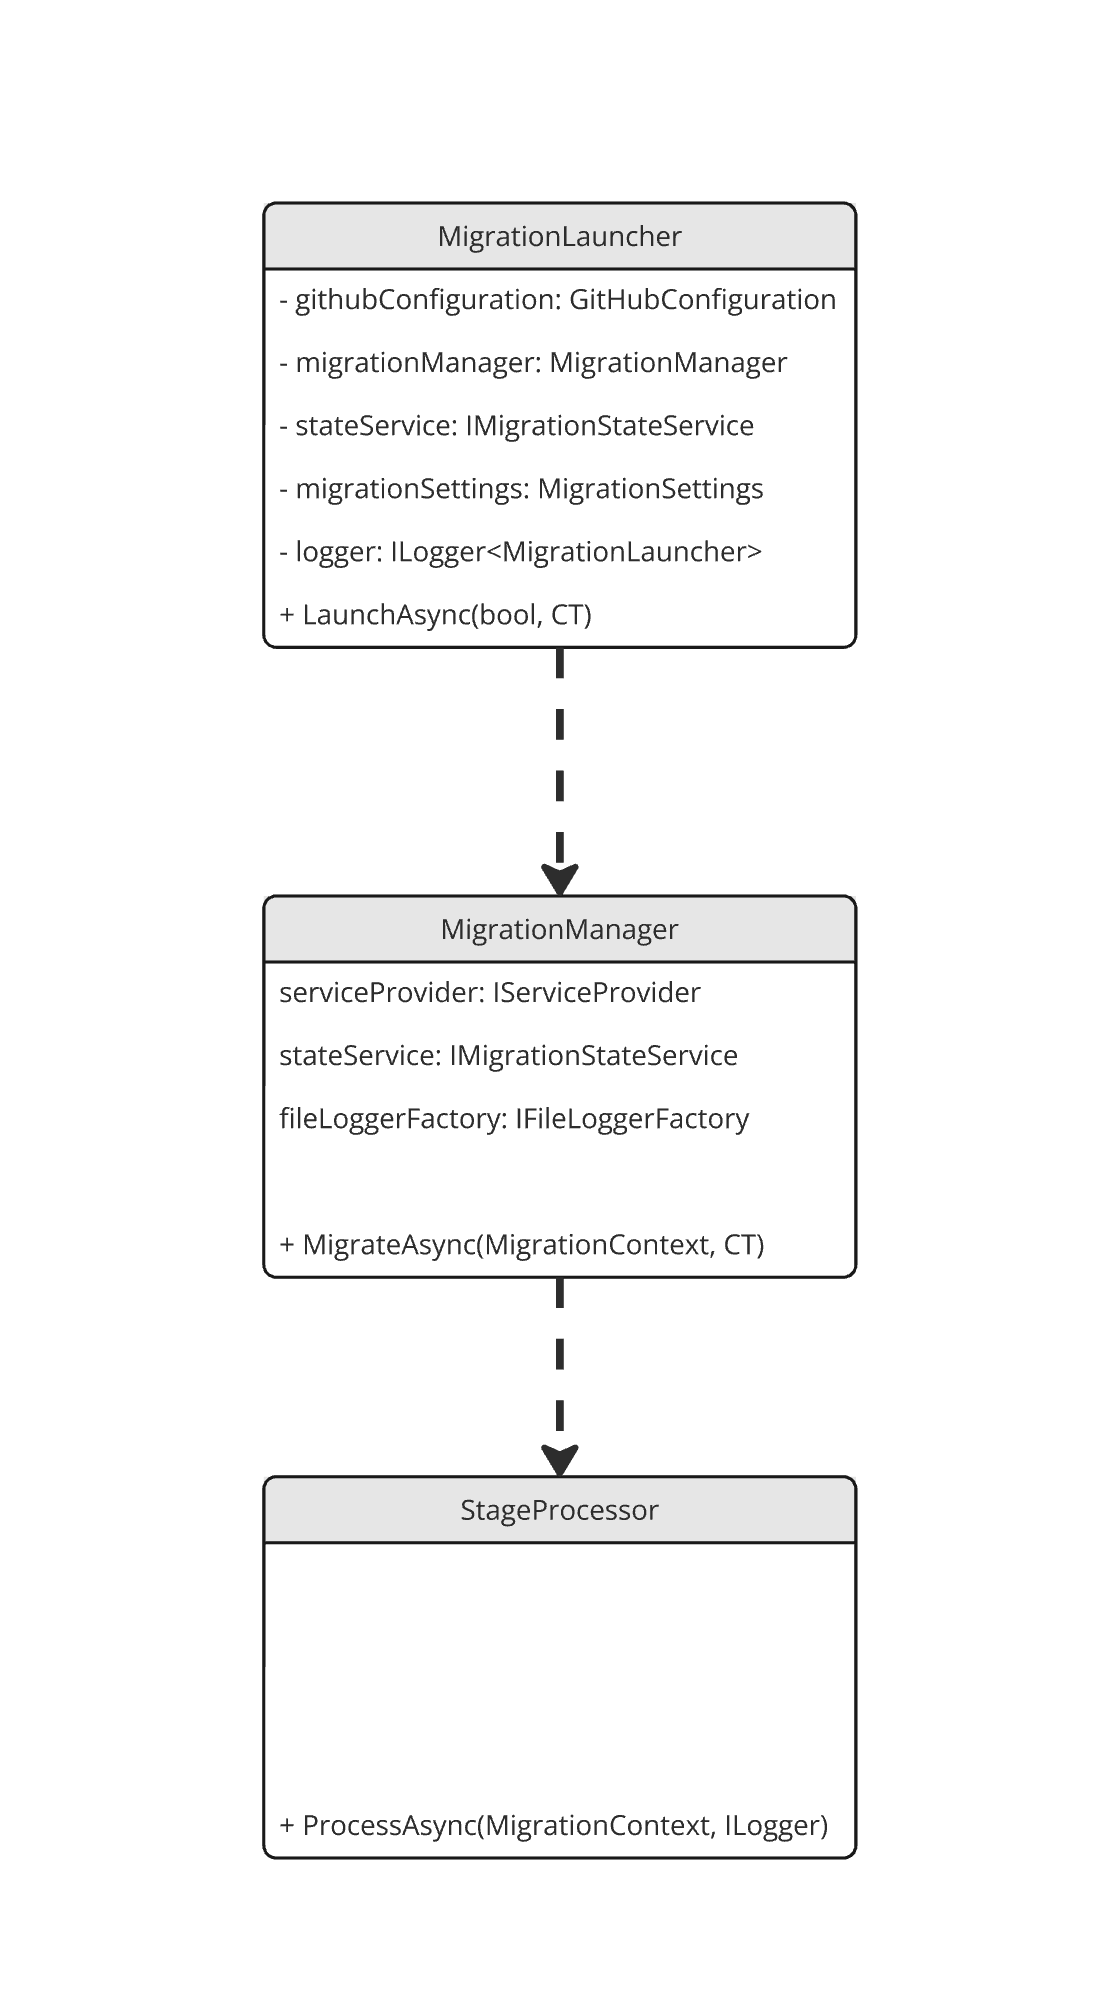
\includegraphics[width=10cm]{img/gitlab-migrator-app-architecture}
  \caption{Архитектура мигратора}
  \label{fig:gitlab-migrator-app-architecture}
\end{figure}

Поскольку пользователь может в любой момент завершить работу консольного приложения, необходимо локальное хранилище для сохранения состояния миграции.
Для этого был выбран YAML-файл: причина была в простоте и отсутствии необходимости более комплексных решений, например, отдельной базе данных.
Сам файл содержит всю необходимую информацию о репозиториях (Рис. \ref{fig:migration-state-file}).
Для создания и поддержания актуальности этого файла используется отдельная консольная команда,
которая взаимодействует с сетевым интерфейсом сервиса GitHub для получения данных о репозиториях и сетевым интерфейсом сервиса Google Sheets для получения информации о принадлежности репозитория определенной команде организации.
Актуализация данных происходит автоматически с помощью запланированной задачи, которая периодически запускает команду и фиксирует изменения в репозитории.

\begin{figure}[H]
  \centering
  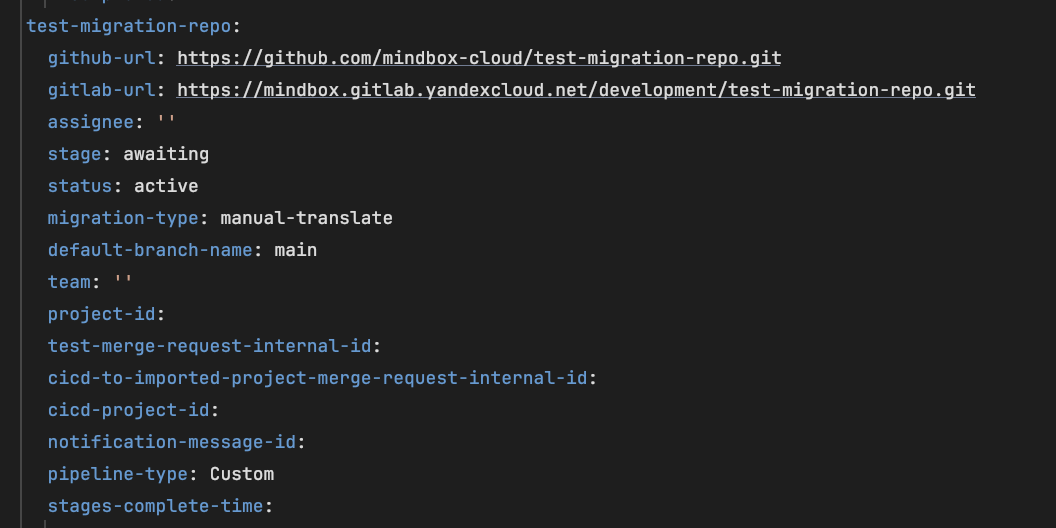
\includegraphics[width=12cm]{img/migration-state-file}
  \caption{Пример данных в YAML-файле для репозитория}
  \label{fig:migration-state-file}
\end{figure}

Принцип работы мигратора при переносе репозиториев следующий:
\begin{enumerate}
  \item \texttt{MigrationLauncher} выбирает репозитории, которые пользователь отметил для переноса (вписал свое имя в поле \texttt{assignee}).
  \item Далее этот класс запрашивает данные из общего YAML-файла и создает соответствующее количество экземпляров \texttt{MigrationManager},
        каждый из которых отвечает за миграцию одного репозитория.
  \item \texttt{MigrationManager} с помощью \texttt{IServiceProvider} находит \texttt{IStageProcessor},
        соответствующий текущему этапу миграции, и запускает его.
  \item После выполнения этапа процессор возвращает следующий шаг или ошибку, которую необходимо обработать и записать.
\end{enumerate}

Для удобства работы с промежуточными записями работы программы была реализована обертка над \texttt{ILogger},
которая перенаправляет записи в отдельный файл.

Всего в миграторе 30 шагов.
Каждый шаг содержит идемпотентную логику, связанную с определенным аспектом переноса проекта с GitHub на GitLab.
Это полезно в случае, если работа мигратора прерывается на середине какого-либо шага, то при следующем запуске сторонние эффекты предыдущих запусков не будут накапливаться, и результат будет таким же, как если бы прерывания не было.
Таким образом несколько разработчиков, даже без глубокого знания GitLab и самого мигратора, могут быстро и качественно выполнять миграцию.
В связи с этим каждый шаг достаточно атомарен и обрабатывает небольшую логику.
При этом шаги реализованы как сервисы в единственном экземпляре, что позволяет использовать инъекцию зависимостей.

Шаги миграции разделены на три фазы:
\begin{enumerate}
  \item Фаза переноса конфигураций конвейера в GitLab;
  \item Проверка корректности конвейера на уровне запроса на слияние;
  \item Полноценный импорт репозитория из GitHub с его архивацией и последующим слиянием перенесенной конфигурации конвейера.
\end{enumerate}

Далее описаны общие шаги мигратора в каждой из фаз.

\section{Фаза портирования конвейера в GitLab и проверка корректности на уровне запроса на слияние} \label{sec:first-and-second-phases}
Изначально вторая фаза включала проверку корректности конвейера как на уровне запроса на слияние, так и на уровне создания новой версии сервиса.
Однако в текущей реализации проверка корректности конвейера выпуска (release) была перенесена в третью фазу, что сделало вторую фазу менее объемной.
Поэтому здесь она рассматривается совместно с первой фазой.

\begin{enumerate}
  \item Уведомление в мессенджер о начале портирования конвейера репозитория.
        Канал отправки зависит от указанной команды;
  \item Локальное клонирование репозитория с префиксом \texttt{*cicd} и создание ветки для тестирования;
  \item Замена источника пакетов NuGet\cite{nuget} на GitLab в файле конфигурации и всех упоминаний GitHub в YAML и Docker файлах;
  \item Опциональная трансляция \emph{скелета} конвейера.
        Выполняется только при выборе определенного \texttt{MigrationType};
  \item Отображение подсказок в консоли, зависящих от типа репозитория.
        Например, для библиотек может быть предложено увеличить минорную версию, а для сервисов — заменить старое хранилище образов.
        Подсказки добавляются с помощью \texttt{KeyedSingleton}, что позволяет повторно использовать их в разных шагах без нарушения принципа избежаний дубликатов;
  \item Автоматическое создание запросов на слияния из ветки для тестирования в основную ветку.
        Проверяется результат выполнения конвейера.
        Ожидание завершения конвейера реализовано через возвращение шагом самого себя, что позволяет мигратору периодически проверять статус;
  \item При падении конвейера мигратор возвращается к шагу \texttt{merge\_request\_pipeline\_changes\_required}, чтобы пользователь мог исправить ошибки и повторить проверку.
        Для этого необходимо внести изменения в ветку для тестирования и перезапустить мигратор.
        Шаги с таким поведением помечены специальным атрибутом, что позволяет \texttt{MigrationManager} завершить работу при переходе на такой шаг.
\end{enumerate}

\section{Полноценный импорт репозитория из GitHub с архивацией и слиянием перенесенной конфигурации конвейера} \label{sec:third-phase}

\begin{enumerate}
  \item Уведомление в мессенджер о начале импорта репозитория, а в конце работы и о завершении миграции.
        Канал отправки зависит от указанной команды;
  \item Архивирование репозитория в GitHub для предотвращения рассинхронизации с GitLab;
  \item Импорт репозитория из GitHub в GitLab и ожидание завершения процесса.
        Он выполняется с помощью ранеупомянутого встроенного инструмента GitLab;
  \item Шаг с подсказками, аналогичный предыдущему, но с другим набором рекомендаций;
  \item Автоматическое обновление настроек проекта в Octopus Deploy, включая изменение различных переменных шагов, например, источник получаемого кода на встроенный вариант вместо GitHub;
  \item Создание запроса на слияние в импортированном репозитории на основе ранее протестированной ветки.
        Поскольку конвейер уже был проверен, он сразу сливается с мигратором, и мигратор отслеживает результат выполнения конвейера выпуска или добавлений изменений в основную ветку;
  \item При неудачном выполнении конвейера изменения откатываются, и мигратор возвращается к шагу \texttt{release\_pipeline\_changes\_required}.
        Пользователь должен исправить ошибки в ветке для тестирования и перезапустить мигратор;
  \item Перенос настроек, которые не поддерживаются встроенным импортом: настройки репозитория, например: политики слияния, защищенные ветки и множества правил (rulesets), отсутствующие в GitLab и требующие ручного сопоставления с доступными настройками.
        Также выполняется настройка прав доступа для групп и отдельных пользователей.
  \item Разархивация репозитория в GitHub и переключение его в режим чтения для всех пользователей.
        Необходимо, так как в компании есть автоматизация, основанная на Terraform модуле, которому необходимо, чтобы репозиторий не был заархивирован.
\end{enumerate}

%% TODO: conclusion
